\documentclass[11pt]{article}
\usepackage[margin=1in]{geometry}
\usepackage[numbers,sort&compress]{natbib}
\usepackage{amsmath,amssymb}
\usepackage{graphicx}
\usepackage{booktabs}
\usepackage{url}
\usepackage[hidelinks]{hyperref}

\begin{document}

\title{ShieldCall: Dual-stream telephony sensing and a belief-state defense agent for vishing and vocoded-speech threats}
\author{Vubangsi Mercel\\
{\small Independent researcher \quad\texttt{vmercel@gmail.com}}}
\date{}
\maketitle

\noindent\textit{Intended venue.} Computers \& Security (Elsevier), with Information Fusion as an alternative. This is a journal manuscript, not an arXiv note. Claims are limited to measurements in the companion repository.

\vspace{0.6em}
\noindent\textbf{Highlights}
\begin{itemize}
\item A scam-stage tracker outperforms high-precision keywords on held-out paraphrases (AUC $0.88$ vs $0.42$) while isolated-keyword benign traps remain low ($0.23$).
\item Operational call threat is defined as the disjunction of hostile language and vocoded production; disagreement-aware fusion raises complementary-cell recall from $0.30$ to $1.00$ at a documented false-alarm cost.
\item A belief-state agent treats detectors as sensors and spends an interruption budget as experiments; it warns on human social engineering and does not waste a nonce on a live speaker.
\item Stage-aligned production change is posed as a timing statistic for mid-call handoffs, validated on synthetic point processes (AUC $1.00$), and \emph{not} supported on pulse-formant splices into Mini LibriSpeech (AUC $0.47$).
\item Lightweight residual features detect an easy pulse-formant vocoder after bandlimiting and fail on LPC (narrowband AUC $0.49$). Neural TTS and ASVspoof numbers are not claimed.
\end{itemize}

\begin{figure}[h]
\centering
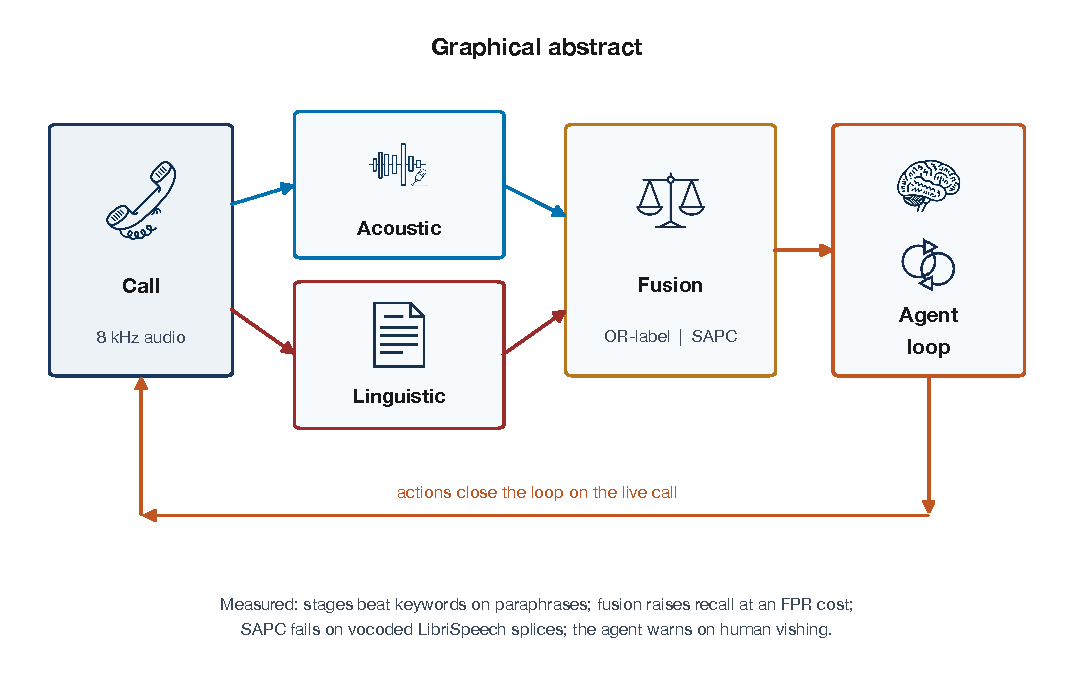
\includegraphics[width=0.95\textwidth]{figures/graphical_abstract.pdf}
\caption{Graphical abstract. The pipeline emits sufficient statistics. A discrete-hypothesis agent chooses actions. The figure states what is measured, including the failed audio handoff test.}
\label{fig:ga}
\end{figure}

\begin{abstract}
Telephone fraud increasingly mixes social-engineering scripts with synthetic or vocoded speech. Published countermeasures usually address one stream: anti-spoofing on whole utterances, or text classifiers on transcripts. Late fusion by weighted averaging treats the streams as redundant rather than complementary, and it cannot represent a mid-call production switch timed to a harvest ask. This paper describes ShieldCall, a streaming system that scores linguistic fraud-intent and acoustic production artifacts on a shared eight-kilohertz timeline, fuses them under an operational disjunction label, and hands the resulting sufficient statistics to a belief-state defense agent. The agent never observes waveforms or transcripts. It maintains a distribution over five call hypotheses and selects among monitor, challenge, warn, escalate, adapt, and abstain by expected information gain minus interruption cost. Likelihoods in the agent are heuristic; we do not claim a fitted Bayesian network or an improvement in equal error rate.

On eighty-six author-written English scripts, a discourse-stage tracker recovers held-out paraphrases that collapse a keyword baseline (AUC $0.883$ versus $0.417$). On speaker-disjoint Mini LibriSpeech, a pulse-formant vocoder is separated after telephone-band filtering (EER $0$, $n{=}20$), whereas low-order LPC is not (narrowband AUC $0.49$). Under the operational label ``threat if scam language or vocoded voice,'' disagreement-aware fusion reaches complementary-cell recall $1.00$ against $0.30$ for a naive weighted sum, with safe-cell false-positive rate $0.40$ versus $0.00$ at threshold $0.5$ ($n{=}40$). Adaptive conformal inference tracks a coverage target of $0.90$ with empirical coverage $0.885$ on a synthetic prevalence-shift stream. A timing statistic for stage-aligned production change ranks perfectly on synthetic point processes and does not separate matched-mix vocoded splices. The contribution is a formulated problem, a measured sensor stack, a measured agent policy shape, and public negative results. It is not a state-of-the-art anti-spoofing encoder.
\end{abstract}

\noindent\textit{Keywords:} vishing; voice spoofing; telephone channel; score fusion; change-point; conformal inference; intelligent agent; active sensing.

\section{Introduction}

Impersonation and payment-harvesting calls remain a first-order consumer-protection problem~\cite{ftc2024sentinel}. Two technical facts make the problem different from keyword spotting on a clean recording. First, a live human can walk a victim through authority, urgency, credential harvest, and prepaid-card payment without ever using a neural vocoder. The incriminating evidence is then the \emph{script}. Second, when a voice is synthetic, the cues that laboratory anti-spoofing systems exploit are distorted by $\mu$-law quantization, $300$--$3400$\,Hz bandlimiting, and packet-loss concealment~\cite{zhang2021channel,todisco2019asvspoof}. A third fact is now operational: real-time voice conversion can be inserted \emph{during} a call, so that rapport is human and the harvest is not. Whole-utterance scores average those regimes away.

The literature has strong answers to adjacent questions. The ASVspoof series and successors such as AASIST and RawNet2 address logical-access synthesis and conversion under controlled protocols~\cite{todisco2019asvspoof,wang2020asvspoof,jung2022aasist,tak2021end}. PartialSpoof asks whether any segment of an utterance is fake~\cite{zhang2021partial,zhang2023partialspoof}. Dialogue-act tagging is a mature NLP task~\cite{stolcke2000dialogue}. Contact-centre products fuse audio and text by weighted scores. None of those lines, as published, jointly (i) treat telephony as a first-class evaluation condition, (ii) label a call as a threat if \emph{either} stream is hostile, (iii) spend an interruption budget as a sequential experiment, and (iv) pose---and attempt to falsify---a timing hypothesis that a production change-point coincides with a harvest-class stage.

This paper studies that joint problem with a system called ShieldCall. The detector stack is a sensor: it emits synthetic probability, fraud probability, a timing statistic, a coverage-gap, a regime tag, and an uncertainty interval. A defense agent updates a discrete belief and acts. The agent is not a large language model. Putting an LLM on the transcript would reintroduce privacy cost, latency, and unmeasured decision making. The agent is a Russell--Norvig process with five hypotheses and six tools.

The research questions are stated so they can fail.

\begin{quote}
\textbf{RQ1.} Does a streaming scam-stage tracker add detection on paraphrases that avoid high-precision keywords, without inflating isolated-keyword benign traps?

\textbf{RQ2.} If a call is a threat whenever language is hostile \emph{or} production is vocoded, does disagreement-aware fusion recover complementary cells that a weighted sum misses, and at what false-alarm cost?

\textbf{RQ3.} Can a residual-plus-prototype scorer, fit speaker-disjoint on Mini LibriSpeech, separate a pulse-formant vocoder and an LPC vocoder after telephone-band filtering?

\textbf{RQ4.} Does a Gaussian coupling of an estimated production change-point to harvest-class stage times rank aligned handoffs above duration-matched unaligned splices?

\textbf{RQ5.} Does a belief-state agent, given only those sufficient statistics, produce different action traces for benign, human-vishing, and handoff-like percept sequences, without using an LLM?
\end{quote}

The answers, in preview, are yes (RQ1), yes with a quantified cost (RQ2), yes on pulse-formant and no on LPC (RQ3), no on the LibriSpeech construction despite a clean synthetic check (RQ4), and yes on scripted percepts (RQ5). We treat the RQ4 failure as a result, not as a prompt to retune until the test passes.

\section{Related work}

\subsection{Anti-spoofing and telephony}
ASVspoof established community protocols for logical access and replay~\cite{todisco2019asvspoof,wang2020asvspoof}. Competitive systems use self-supervised front ends and graph or raw-waveform backends~\cite{jung2022aasist,tak2021end}. Those systems are the right comparison for neural text-to-speech and voice conversion. We do not replace them and we do not report ASVspoof equal error rates. Channel mismatch is a documented failure mode~\cite{zhang2021channel}. Our telephone-band simulator is a classical DSP chain (bandlimit, $\mu$-law, noise, packet loss with concealment). It is a stress test, not a learned generative model of the public switched network.

PartialSpoof constructed utterances in which only some segments are fake and showed that counters trained on fully spoofed data degrade~\cite{zhang2021partial,zhang2023partialspoof}. That line asks whether any frame is synthetic. It does not ask whether the fake onset is timed to a vishing stage, and it does not consume a linguistic stream.

\subsection{Vishing and discourse}
Applied vishing detectors typically classify transcripts or average an audio score with a text score. Dialogue-act models assign speech to acts such as request and statement~\cite{stolcke2000dialogue}. Professional scam calls are not a bag of words; they progress through greeting, claimed authority, invented problem, urgency, harvest, payment, secrecy, and threat. A keyword list that fires on ``IRS'' and ``gift card'' fails when those strings are paraphrased, and it fires on benign mentions of a bank holiday. The gap we test is whether a small stage machine with a broader emission lexicon recovers paraphrases while remaining quiet on isolated-keyword traps. We do not claim to have invented dialogue-act tagging.

\subsection{Fusion and uncertainty}
Late fusion by weighted sum or stacking is standard multimodal practice. If the operational label is a logical OR, averaging is the wrong combination: a vocoded probe with mild language is diluted, and a human vishing call is diluted by a low synthetic score. Disagreement regimes (safe, social engineering, spoof probe, dual) are a taxonomy, not Pearl causality. We compare rule-based floors against naive sum, unimodal scores, and logistic regression on the same two scalars.

Conformal prediction supplies finite-sample coverage under exchangeability~\cite{angelopoulos2023gentle}. For streams that shift, Gibbs and Cand\`es proposed adaptive conformal inference~\cite{gibbs2021aci}. We implement that recursion on labeled scores. An exponential-moving-average band remains in the code as a heuristic; it is not ACI and is not used for the coverage number in this paper.

\subsection{Agents}
A rational agent maps percepts to actions under a utility~\cite{russell2010aima}. Large language model agents that plan over raw transcripts are a current fashion. For a telephone call they are the wrong first design: they observe too much, they are unmeasured, and a human social engineer will pass a spoken nonce that a vocoder should fail. Our agent therefore sees only sufficient statistics, holds a five-atom belief, and treats a liveness challenge as a costly experiment whose value depends on the current hypothesis. We do not claim Lindley-optimal design; the likelihoods are declared by hand.

\section{Problem formulation}

Let a call be a stream of frames at hop $\Delta=10$\,ms on an $8$\,kHz axis, together with timestamped transcript fragments. At time $t$ the sensor produces $s_t\in[0,1]$ (synthetic probability), $f_t\in[0,1]$ (fraud probability), a change-point estimate $\hat\tau$ when available, stage times $\{t_k\}$ in a harvest-class set $\mathcal{H}$, a coverage gap $g_t$, and an interval $[L_t,U_t]$.

\noindent\textbf{Operational threat.}
A labeled evaluation call is a threat if and only if its language is a scam script or its audio is vocoded (or both). It is safe only if the voice is bona fide and the script is benign.

\noindent\textbf{Stage-aligned production change.}
Let $C=\max_{t_k\in\mathcal{H}}\exp\bigl(-(t_k-\hat\tau)^2/(2\sigma^2)\bigr)$ with $\sigma=0.45$\,s. Under a circular-shift null of $\hat\tau$ on the call duration $T$, $p=(1+\#\{C_{\mathrm{null}}\ge C\})/(B+1)$. The SAPC score is $C(1-p)$.

\noindent\textbf{Call hypotheses.}
The agent entertains a mutually exclusive set $H=\{\mathrm{benign},\,\mathrm{SE},\,\mathrm{synthetic},\,\mathrm{handoff},\,\mathrm{unknown}\}$ for the current call. A percept updates a distribution $p(H)$. An action $a$ is chosen to approximately maximise expected information gain minus $\lambda_{\mathrm{c}}\mathrm{cost}(a)$ minus a delay penalty when threat mass is high and $a$ is passive.

Novelty, if any, lives in these definitions plus the measurements, not in residual spectral features, CUSUM, or prototypical memory, all of which have decades of prior art~\cite{page1954cusum,snell2017prototypical,griffin1984signal}.

\section{System}

Fig.~\ref{fig:ga} and Fig.~\ref{fig:arch} summarise the architecture. Incoming audio is resampled and optionally passed through the telephone-band simulator, then framed. The acoustic path computes a residual fingerprint after a least-squares harmonic model and a prototype-memory score. The linguistic path blends high-precision patterns with a hidden Markov stage tracker. Fusion emits a risk, a regime, SAPC fields, and an ACI or heuristic interval. The agent consumes those fields only.

\begin{figure}[t]
\centering
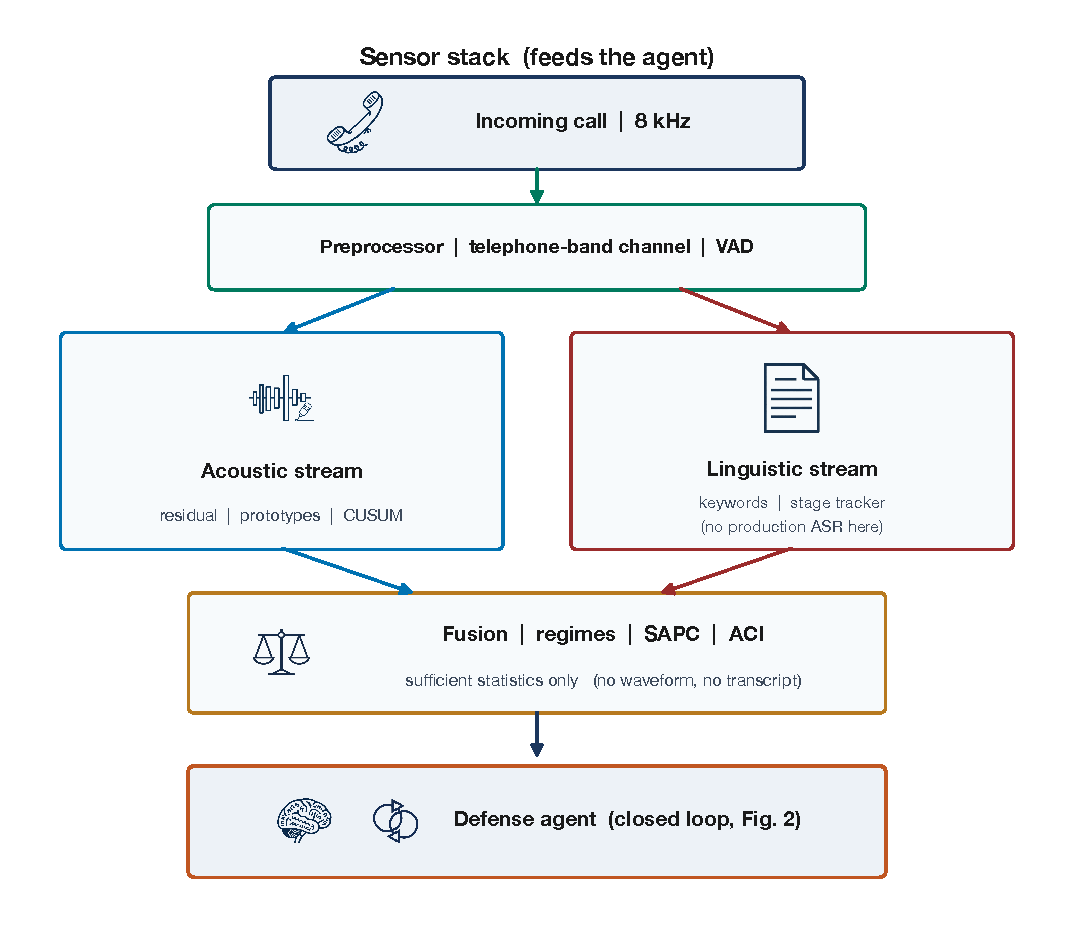
\includegraphics[width=0.98\textwidth]{figures/architecture_pipeline.pdf}
\caption{Sensor stack. Fusion outputs sufficient statistics. The bottom box is the defense agent, not a second classifier.}
\label{fig:arch}
\end{figure}

\begin{figure}[t]
\centering
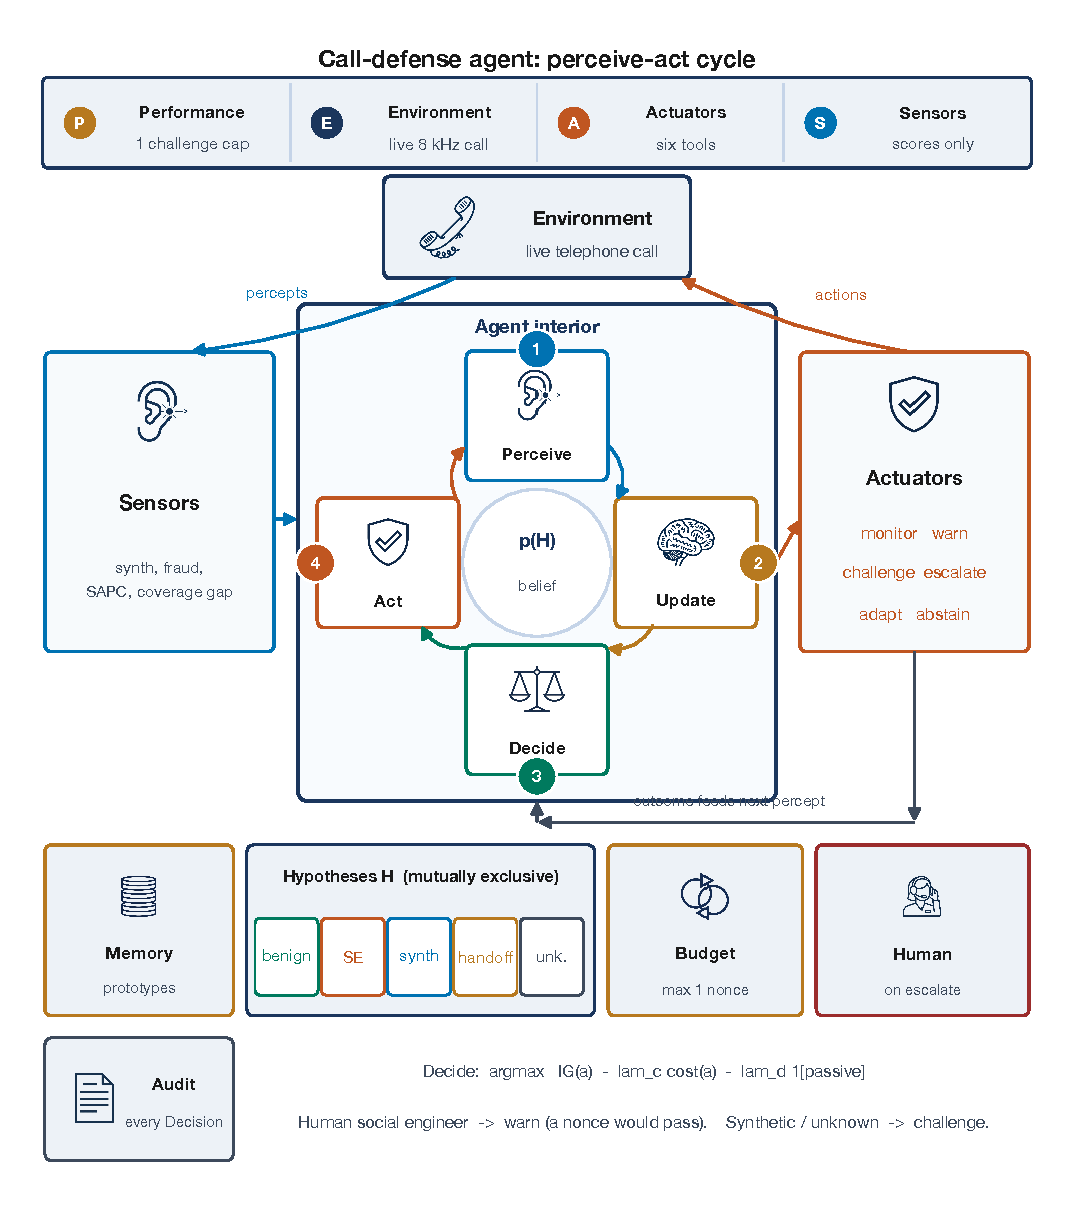
\includegraphics[width=0.98\textwidth]{figures/agent_loop.pdf}
\caption{Call-defense agent as a closed perceive--act cycle. PEAS describes the task. Sensors emit scores only. The interior updates $p(H)$ and chooses an action by information gain minus interruption cost. Actuators close the loop on the live call. A social engineer is warned, not challenged.}
\label{fig:agent}
\end{figure}

\begin{figure}[t]
\centering
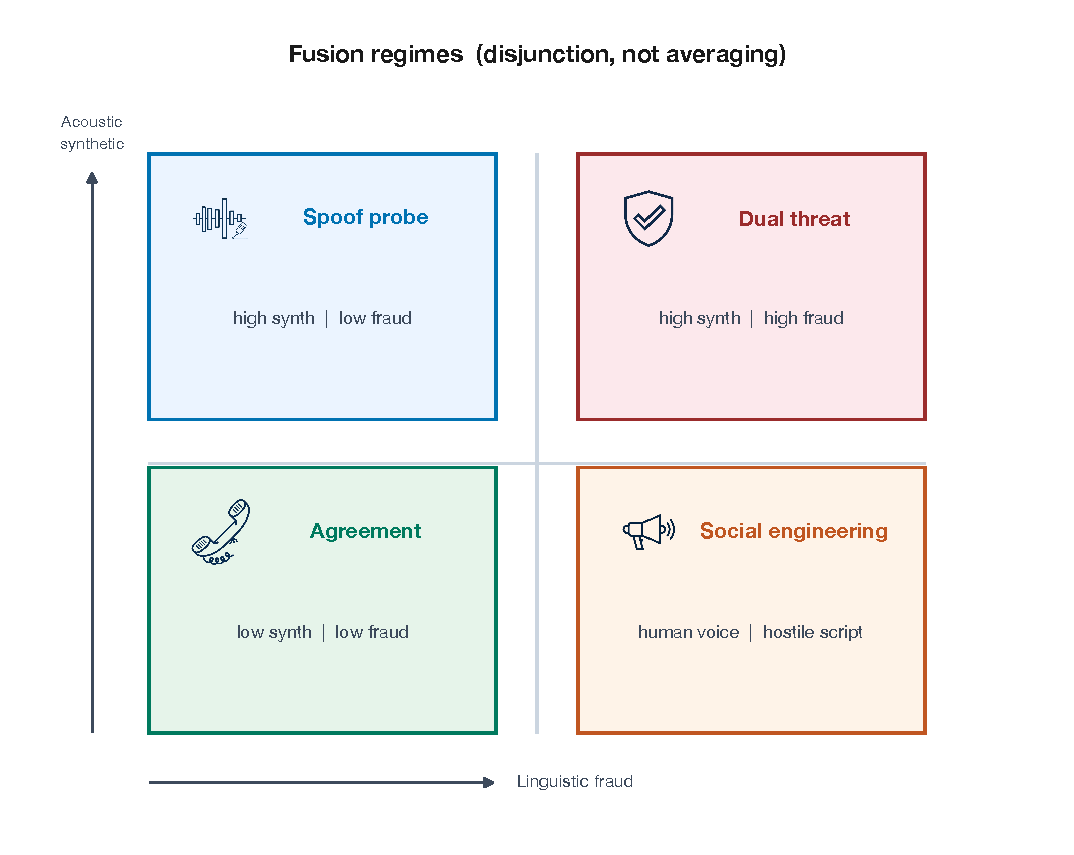
\includegraphics[width=0.92\textwidth]{figures/cscf_regimes.pdf}
\caption{Four disagreement regimes. The operational label is an OR over the two axes.}
\label{fig:regimes}
\end{figure}

\begin{figure}[t]
\centering
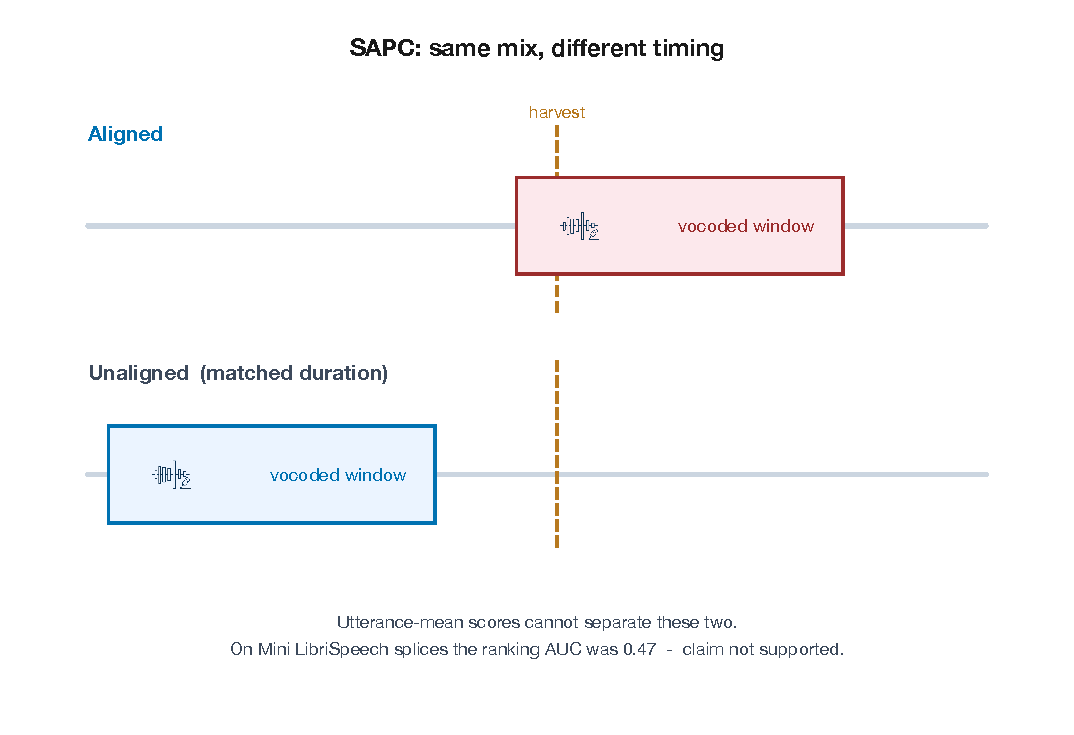
\includegraphics[width=0.92\textwidth]{figures/sapc_timing.pdf}
\caption{SAPC construction. The vocoded duration is matched; only alignment to the harvest stage differs. The LibriSpeech splice test did not support the timing claim.}
\label{fig:sapc}
\end{figure}

\subsection{Operational architecture}
The library is not a telephone switch. Fig.~\ref{fig:deploy} is the designed placement: a session-border controller keeps SIP and RTP on the media path and forks an eight-kilohertz copy to a ShieldCall worker. One in-memory session holds one pipeline and one agent for the life of a \texttt{call\_id}. Workers scale horizontally by call identity. If a worker is at capacity it \emph{sheds}: it spends no CPU and emits only \texttt{monitor}, so the call continues. If the worker dies, in-call belief is lost and RTP is unaffected. Automatic speech recognition sits behind a circuit breaker; the acoustic path continues. These contracts live in \texttt{shieldcall.runtime} and are unit-tested. They are not a carrier deployment.

On the evaluation host a frame costs about $6.2$\,ms against a $10$\,ms hop (realtime factor $\approx 1.6$). At seventy percent utilisation that is on the order of one full-rate call per core. Capacity is $N_{\mathrm{call}}/N_{\mathrm{core}}=(t_{\mathrm{hop}}/t_{\mathrm{frame}})\rho$. Cost is vCPU, not GPU. Neural vocoder detectors would change that bill; we do not run one.

\begin{figure}[t]
\centering
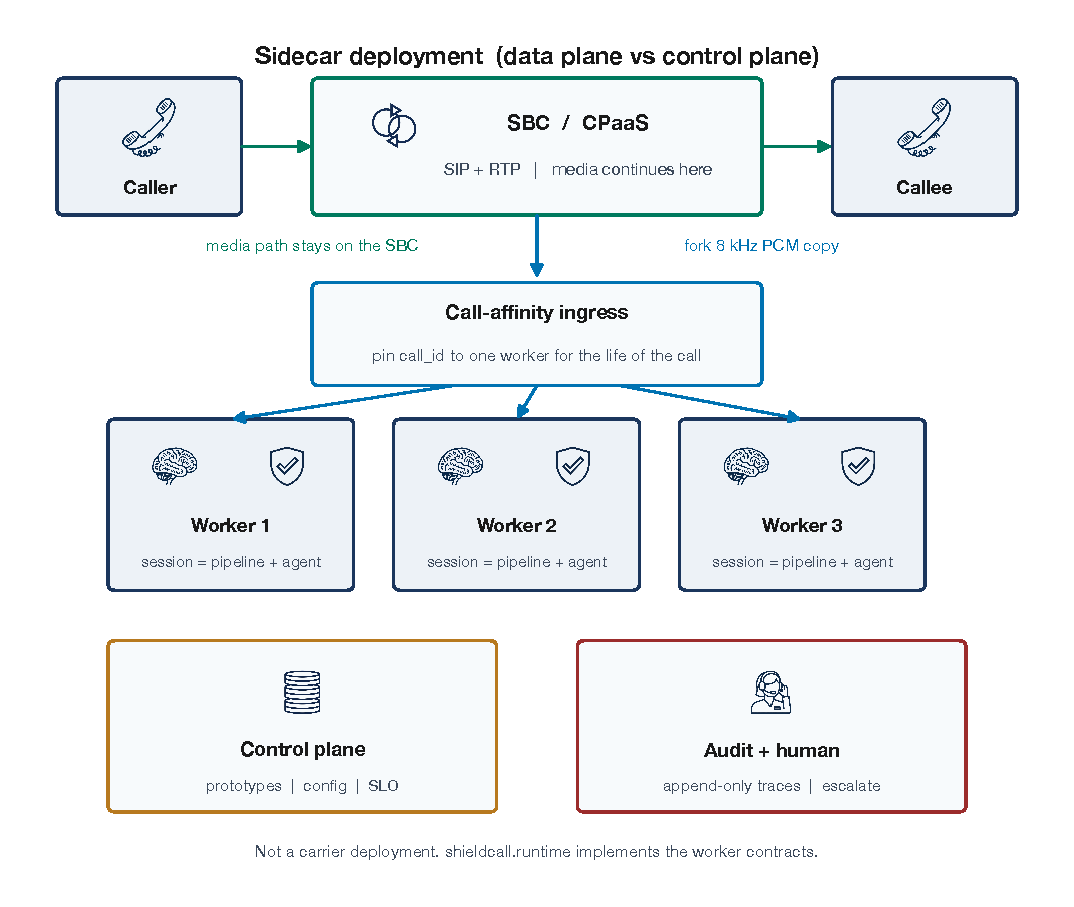
\includegraphics[width=0.98\textwidth]{figures/deployment_sidecar.pdf}
\caption{Sidecar placement. The call is the scale unit. Media does not hairpin through the detector.}
\label{fig:deploy}
\end{figure}

\begin{figure}[t]
\centering
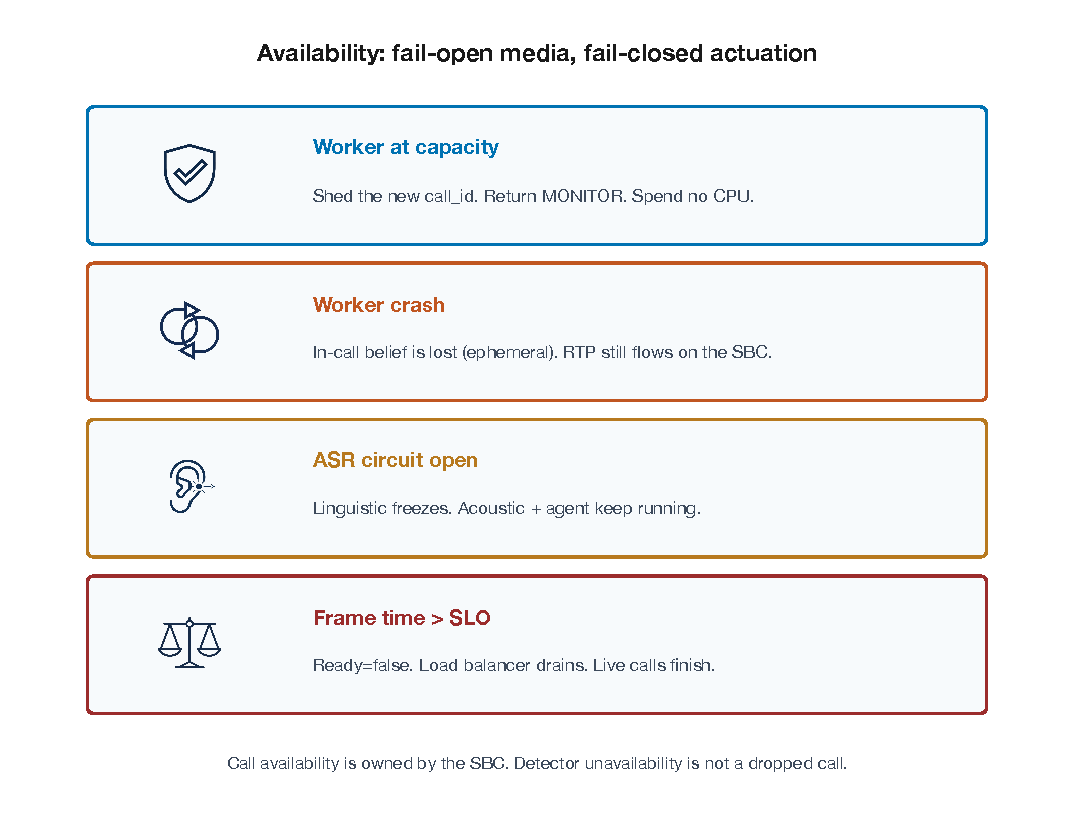
\includegraphics[width=0.92\textwidth]{figures/reliability_failopen.pdf}
\caption{Failure policy. Call availability is owned by the SBC. Detector unavailability must not drop the call; actuation fails closed.}
\label{fig:rel}
\end{figure}

\section{Methods}

\subsection{Acoustic scoring}
Each $25$\,ms speech frame is decomposed with a harmonic model. Residual energy ratio, spectral flatness, excess kurtosis, Hilbert-envelope modulation, harmonic-to-noise ratio, phase irregularity, and an upper-band peak-to-median ratio are concatenated with coarse spectral descriptors into a $64$-dimensional vector. Prototype memory stores class-conditional means and scores by a softmax over RMS Mahalanobis distances. Memory is fit on labeled training clips; Gaussian bootstrap priors are not used in reported numbers. Page CUSUM~\cite{page1954cusum} watches $s_t$ online. Offline, $\hat\tau$ maximises the absolute two-window mean difference.

Two vocoders are used as \emph{controlled} production models, not as stand-ins for HiFi-GAN. Pulse-formant is an impulse train at estimated $F_0$ through three analog-style formants (easy). LPC is a low-order vocoder with pulse or noise excitation (hard). Griffin--Lim~\cite{griffin1984signal} is implemented but is not the primary reported condition.

\subsection{Linguistic scoring}
Keyword groups are high-precision English regular expressions. The stage tracker is an HMM whose emissions are a broader lexicon and whose transitions prefer forward progression through greeting, authority, problem, urgency, harvest, payment, secrecy, and threat. The path score mixes progression depth with mean per-step log-likelihood. There is no production automatic speech recognizer in the experiments; fragments are injected. The linguistic numbers therefore isolate language modeling, not recognition error.

\subsection{Fusion}
Let $s$ and $f$ denote the current synthetic and fraud probabilities. A naive baseline is $0.4s+0.6f$. ShieldCall uses a confidence-weighted blend, a social-engineering floor when $f$ is high and $s$ is not, and a spoof-probe floor when $s$ is high and $f$ is not, gated on acoustic confidence so that uncertain residual scores do not force probes. Counterfactuals re-evaluate the same function with $f=0$ or $s=0$. This is rule-based fusion.

\subsection{SAPC}
Harvest-class stages are harvest, payment, threat, and secrecy. Coupling uses the first estimated change-point only, because frame-level jitter otherwise saturates the kernel. The permutation null circularly shifts that time. The hypothesis is tested by constructing two splices with the same vocoded fraction: onset at the harvest fraction versus onset at the opposite end of the call.

\subsection{ACI}
On a labeled stream, residuals $|s-y|$ update
\[
\alpha_{t+1}=\Pi_{[\alpha_{\min},\alpha_{\max}]}\bigl(\alpha_t+\gamma(\alpha-\mathrm{err}_t)\bigr),
\]
with interval half-width the empirical $(1-\alpha_t)$-quantile of past residuals~\cite{gibbs2021aci}. Coverage is empirical.

\subsection{Agent}
The prior is peaked on benign ($0.80$), because most calls are legitimate. Each percept multiplies a hand-written likelihood and mixes with inertia $0.65$. Challenge-failure probabilities are $0.06$ (benign), $0.10$ (social engineering), $0.82$ (fully synthetic), $0.55$ (handoff), $0.40$ (unknown). The planner scores each action by expected entropy reduction minus cost minus delay. A hard constraint forbids a challenge while the mode is benign and threat mass is below $0.30$. At most one challenge is issued per call. Rationale strings are templates. No LLM is imported on the decision path.

\section{Experimental design}

Sine-wave unit tests exist in the repository and are not scientific results. Mini LibriSpeech \texttt{dev-clean-2}~\cite{panayotov2015librispeech} provides bona fide speech. Splits are speaker-disjoint. ASVspoof was not present; a loader is implemented and unused. Author-written scripts ($48$ train, $38$ held-out) include paraphrases and isolated-keyword traps. They are not a sample of real victims.

Fusion uses the operational OR label and $n{=}40$ cells (safe, social engineering, spoof probe, dual) on pulse-formant audio with held-out scripts. Logistic regression is fit on a grid of synthetic probabilities crossed with training-script fraud scores, not on test audio.

SAPC audio uses stitched $\sim$10\,s calls, a vocoded window of relative length $0.34$, and $n{=}6$ speaker pairs. Mix match is a gate: mean $s$ must agree within $0.12$ before ranking is interpreted. Synthetic SAPC uses forty aligned versus unaligned point-process draws.

Agent evaluation uses scripted percept sequences, not live audio: a dentist reminder, a human IRS-style vishing path, and a handoff-like path. The measured object is the action trace.

Sample sizes are small. We do not report $p$-values on $n{=}6$ as evidence of absence beyond the ranking AUC itself.

\section{Results}

\subsection{RQ1: language}
Table~\ref{tab:ling} and Fig.~\ref{fig:ling} show that on canonical training lines the keyword list is already strong (AUC $0.929$). On held-out paraphrases it falls below chance (AUC $0.417$, EER $0.583$). Adding the stage tracker recovers AUC $0.883$ and EER $0.106$. Mean fraud probability on held-out isolated-keyword traps is $0.234$. The stage machine is doing work the keyword list cannot do on this corpus. The corpus is author-written English.

\begin{table}[t]
\centering
\caption{Linguistic detection. Traps report mean fraud probability (lower is better).}
\label{tab:ling}
\begin{tabular}{lccc}
\toprule
Condition & $n$ & EER & AUC \\
\midrule
Train, keywords & 48 & 0.104 & 0.929 \\
Train, keywords+stages & 48 & 0.000 & 1.000 \\
Held-out, keywords & 38 & 0.583 & 0.417 \\
Held-out, keywords+stages & 38 & 0.106 & 0.883 \\
Held-out traps (mean score) & 8 & --- & 0.234 \\
\bottomrule
\end{tabular}
\end{table}

\begin{figure}[t]
\centering

\includegraphics[width=0.72\textwidth]{figures/linguistic_auc.pdf}
\caption{Linguistic AUC. The stage tracker is redundant on canonical training lines and necessary on held-out paraphrases.}
\label{fig:ling}
\end{figure}

\subsection{RQ3: acoustics}
Pulse-formant versus bona fide, speaker-disjoint, $n{=}20$, is easy: EER $0.00$ and AUC $1.00$ both clean and after $300$--$3400$\,Hz bandlimiting. That shows the residual front end can fire on robotic excitation after telephone filtering. It does not show neural-TTS detection.

LPC on the same protocol is hard. Clean LPC yielded EER $0.40$ / AUC $0.64$. Narrowband LPC was at chance (EER $0.45$ / AUC $0.49$). Five-shot adaptation of a pulse-formant memory toward LPC reduced unseen LPC EER from $0.50$ to $0.45$. Lightweight residual features, as implemented, are not a substitute for ASVspoof-trained neural countermeasures~\cite{jung2022aasist}.

\subsection{RQ2: operational fusion}
Table~\ref{tab:fuse} and Fig.~\ref{fig:fuse} report the OR-label task. Linguistic-only almost never catches a vocoded call that uses mild language (disagreement recall $0.05$). Naive sum reaches AUC $0.973$ but complementary-cell recall $0.30$ at threshold $0.5$. ShieldCall fusion and logistic regression both reach disagreement recall $1.00$. ShieldCall ranking AUC is $1.000$ on this set of forty cells, with safe-cell false-positive rate $0.40$ versus $0.00$ for the naive sum. The floors buy recall; they are not free. Perfect AUC on $n{=}40$ must not be read as a population claim.

\begin{table}[t]
\centering
\caption{Operational fusion, $n{=}40$. Disagreement recall and safe-cell FPR use threshold $0.5$.}
\label{tab:fuse}
\begin{tabular}{lcccc}
\toprule
System & EER & AUC & Disc.\ rec. & Safe FPR \\
\midrule
Acoustic only & 0.267 & 0.833 & 0.90 & 0.80 \\
Linguistic only & 0.233 & 0.827 & 0.05 & 0.00 \\
Naive sum & 0.100 & 0.973 & 0.30 & 0.00 \\
Logistic regression & 0.083 & 0.993 & 1.00 & 0.50 \\
ShieldCall fusion & 0.000 & 1.000 & 1.00 & 0.40 \\
\bottomrule
\end{tabular}
\end{table}

\begin{figure}[t]
\centering

\includegraphics[width=0.72\textwidth]{figures/fusion_operational.pdf}
\caption{Fusion on operational threat labels. Disagreement rules and logistic regression recover complementary cells; both pay in false positives at the $0.5$ threshold.}
\label{fig:fuse}
\end{figure}

\subsection{RQ4: SAPC}
On synthetic point processes ($n{=}40$ pairs), SAPC pair-win rate and AUC are both $1.00$. That only shows the statistic is ordered when the inputs are clean.

On Mini LibriSpeech splices ($n{=}6$ pairs), mean synthetic probability is matched ($0.580$ vs $0.571$). Coupling AUC for aligned versus unaligned is $0.47$; mean-$s$ AUC is $0.53$; pair-win rate is $0.50$. The mix match holds; the timing claim does not. We did not retune the statistic to force a pass.

\subsection{ACI}
On a $400$-step synthetic stream whose positive prevalence jumps from $0.25$ to $0.75$ at the midpoint, ACI with target $1-\alpha=0.90$ has empirical coverage $0.885$. A frozen $90\%$ quantile fit on the first forty residuals has coverage $0.931$ on the remainder. ACI tracks the target. It is not shown to beat a frozen quantile on this shift.

\subsection{RQ5: agent traces}
Table~\ref{tab:agent} records the scripted percept evaluation. A dentist reminder stays in \texttt{benign} and issues only \texttt{monitor}. A human IRS-style path switches to \texttt{social\_engineering} and issues \texttt{warn}, with zero challenges: a live speaker would pass a nonce. A handoff-like path spends the single challenge at the uncertain midpoint and then \texttt{warn}s once \texttt{handoff} dominates. These traces are the agent result. They are not an EER.

\begin{table}[t]
\centering
\caption{Defense-agent traces on scripted percepts. Likelihoods are heuristic.}
\label{tab:agent}
\begin{tabular}{lllcl}
\toprule
Scenario & Final mode & Action sequence & Challenges & Interpretation \\
\midrule
Benign reminder & benign & monitor $\times 4$ & 0 & Do not interrupt. \\
Human vishing & social\_engineering & monitor, warn $\times 3$ & 0 & Nonce would pass; warn. \\
Handoff-like & handoff & monitor, challenge, warn $\times 2$ & 1 & Probe while uncertain. \\
\bottomrule
\end{tabular}
\end{table}

\section{Discussion}

\subsection{Where novelty sits}
The residual front end, the HMM stage tracker, CUSUM, prototypical memory, and ACI are not new algorithms. Journal novelty, if the manuscript has any, is the \emph{problem} and the \emph{measured policy}, not a new encoder. Specifically: operational threat as a disjunction; a paraphrase test that a keyword list fails and a stage tracker does not; a fusion comparison that reports the false-alarm bill; a timing statistic that is allowed to fail in public; and an agent that refuses to waste a liveness challenge on a human scammer. Reviewers who require a new neural architecture or an ASVspoof leaderboard number will correctly reject the paper on those grounds. Reviewers who require that negative results be suppressed will also reject it. Both reactions are more honest than inflating residual features into a discovery.

\subsection{Threats to validity}
Scripts are author-written and English-only. Audio is Mini LibriSpeech, not telephone speech and not ASVspoof. Pulse-formant is easy by construction. Fusion $n{=}40$ and SAPC $n{=}6$ are small. Agent likelihoods are not learned. There is no ASR in the loop, no user study, and no carrier deployment. The sidecar runtime is an in-process contract, not a measured Kubernetes service. Perfect fusion AUC on a small synthetic OR-task will not survive a larger, noisier set.

\subsection{What would change the claim}
ASVspoof logical access through the same channel simulator, with AASIST or RawNet2 in the same table, would change RQ3. PartialSpoof-style splices with real transcripts would give RQ4 a second chance to fail or succeed. A labeled live-call corpus would test RQ1 and RQ5 outside author-written English. Until then the claims remain as scoped above.

\section{Conclusion}

ShieldCall is a streaming dual-stream sensor plus a budgeted defense agent for telephone-bandwidth fraud. A stage tracker still works when a keyword list is paraphrased away. Disagreement-aware fusion changes the recall and false-alarm tradeoff in the direction an operator would expect, at a price we report. Residual acoustics detect a robotic vocoder after bandlimiting and fail on LPC. Adaptive conformal inference tracks its coverage target on a synthetic shifting stream. A timing statistic for mid-call handoffs works on clean point processes and does not on vocoded LibriSpeech splices. The agent warns on human vishing and spends its nonce where a vocoder might fail. Those sentences are the paper. Sentences about state-of-the-art deepfake detection are not.

\section*{CRediT authorship contribution statement}
Vubangsi Mercel: conceptualization, software, experiments, writing.

\section*{Declaration of competing interest}
The author declares no competing interests.

\section*{Data availability}
Mini LibriSpeech is obtained from OpenSLR~31. Scripts, code, and tabulated results are in the companion repository. ASVspoof is not redistributed; set \texttt{SHIELDCALL\_ASVSPOOF\_ROOT} to enable the unused loader. Reproduce with \texttt{pytest -q}, \texttt{python scripts/run\_paper\_experiments.py}, \texttt{python scripts/run\_handoff\_experiment.py}, \texttt{python scripts/run\_agent\_demo.py}, and \texttt{python scripts/run\_capacity.py}.

\bibliographystyle{unsrt}
\bibliography{references}

\end{document}
